\documentclass[usenames,dvipsnames,10pt]{beamer}

\usetheme{metropolis}
\usepackage{appendixnumberbeamer}

\usepackage{booktabs}
\usepackage[scale=2]{ccicons}

\usepackage{pgfplots}
\usepgfplotslibrary{dateplot}

\usepackage{xspace}
\newcommand{\themename}{\textbf{\textsc{metropolis}}\xspace}

\usepackage{amsmath}
\usepackage{amssymb}

\usepackage{minted}
\usemintedstyle{solarizedlight}
\usepackage{mdframed}
\surroundwithmdframed[linecolor=gray]{minted}

\usepackage{tikz}
\usetikzlibrary{positioning,pgfplots.groupplots,pgfplots.fillbetween,matrix,backgrounds}
\definecolor{sbase3}{HTML}{FDF6E3}
\usepackage{pgfplots}

\newcommand*\GnuplotDefs{
    Binv(p,q)=exp(lgamma(p+q)-lgamma(p)-lgamma(q));
    beta(x,p,q)=p<=0||q<=0?1/0:x<0||x>1?0.0:Binv(p,q)*x**(p-1.0)*(1.0-x)**(q-1.0);
}

\pgfmathdeclarefunction{gauss}{3}{%
  \pgfmathparse{1/(#3*sqrt(2*pi))*exp(-((#1-#2)^2)/(2*#3^2))}%
}

\pgfmathdeclarefunction{exppdf}{2}{%
    \pgfmathparse{#2*exp(-#2*#1)}%
}

\subtitle{Implementing iPMCMC in Monad-Bayes}
\title{Interacting Particle Inference and Probabilistic Programming in Haskell}
\date{\today}
\author{Per Engström \\ \footnotesize\em Supervisor: Magnus Lundstedt, Precisit AB \\ Subject reader: Johannes Borgström}
\institute{Uppsala University}

\begin{document}

\maketitle

\begin{frame}{Table of contents}
  \setbeamertemplate{section in toc}[sections numbered]
  \begin{columns}
      \begin{column}{0.5\textwidth}
  \tableofcontents[hideallsubsections,sections={1-4}]
      \end{column}
      \begin{column}{0.5\textwidth}
  \tableofcontents[hideallsubsections,sections={5-7}]
      \end{column}
  \end{columns}

\end{frame}

\section{Background}

\begin{frame}{Goals}
    \begin{itemize}
\item Implement iPMCMC in Monad-Bayes.

\item Compare to existing methods is Monad-Bayes.

\item Evaluate paralellisation.
\end{itemize}
\end{frame}

\subsection{Background}
\label{sub:background}

\begin{frame}{Monad-Bayes}
    \begin{columns}[T,onlytextwidth]
        \column{0.6\textwidth}
        \begin{itemize}
            
            \item Framework for \alert{Haskell} by Sicibor et al. from their paper \emph{``Practical probabilistic programming with monads''}.

\item Functional Language

\item Probabilistic programming
        \end{itemize}

    \column{0.35\textwidth}

    
\includegraphics[width=\textwidth]{images/haskell.png}
    \end{columns}
\end{frame}

\begin{frame}\centering
    
\includegraphics[width=\textwidth]{images/danger.png}
\end{frame}

\begin{frame}{Probabilistic programming}
    \begin{columns}[T,onlytextwidth]
        \column{0.5\textwidth}
        \begin{description} \em
            \item[Stochastic] Events involving randomness
            \item[Inference] Draw conclusions from model
        \end{description}

        \column{0.5\textwidth}
        \begin{itemize}
            \item Combines programming and stochastic modelling

            \item Models as code

            \item Flexible

            \item Expensive inference
        \end{itemize}
    \end{columns}
\end{frame}

\begin{frame}{Bayes' Theorem}\Huge
    \[
        \Pr(A \mid B) = \frac {\Pr(B \mid A) \Pr(A)} {\Pr(B)}
    \] 
\end{frame}

\begin{frame}{Bayes' Theorem}
    \begin{huge}
        
    \[
        \Pr(\theta \mid D) = \frac {\Pr(D \mid \theta) \Pr(\theta)} {\Pr(D)}
    \] 
    \end{huge}

    \begin{align*}
        \theta \quad& \text{Model parameters} \\
        D \quad& \text{Observed data} \\
        \Pr(\theta) \quad& \text{Prior probability} \\
        \Pr(\theta \mid D) \quad& \text{Posterior probability} \\
        \Pr(D \mid \theta) \quad& \text{Likelihood} \\
        \Pr(D) \quad& \text{Marginal likelihood}
    \end{align*}
\end{frame}

\begin{frame}{Intuition}
    \begin{center}
        
\begin{tikzpicture}[]
    \begin{groupplot}[
        group style={columns=2,horizontal sep=3cm},
        height=5cm,
        width=5cm,
        title=Prior probability,
        ymin=0,
        ymax=1,
        axis lines=middle,
        ]
    \pgfplotsset{ticks=none}
    \nextgroupplot
    \addplot[name path=f,red,domain=0:3,samples=100]{exppdf(x,0.5)};
    \path[name path=axis1] (axis cs:0,0) -- (axis cs:3,0);
    \addplot [
        thick,
        color=red,
        fill=red,
        fill opacity=0.05
    ]
    fill between[
        of=f and axis1,
        soft clip={domain=0:3},
    ];

        \nextgroupplot[title=Posterior probability]
        \addplot[name path=g,red,domain=0:3,samples=100]{gauss(x,2,0.5)};
    \path[name path=axis2] (axis cs:0,0) -- (axis cs:3,0);
    \addplot [
        thick,
        color=red,
        fill=red,
        fill opacity=0.05
    ]
    fill between[
        of=g and axis2,
        soft clip={domain=0:3},
    ];
    \end{groupplot}
    \draw[-stealth,shorten <= 5pt, shorten >= 5pt] (group c1r1.east) -- node[above=10pt]{\em Observations} (group c2r1.west);
    \node [below=5pt of group c1r1] {$\theta$};
    \node [below=5pt of group c2r1] {$\theta$};
\end{tikzpicture}
    \end{center}
\end{frame}

\begin{frame}{\emph{Example:} Biased coin flip}
    Suspicious coin. Test it!

    \pause

\alert{Model} coin outcome as $X \sim \operatorname{Bernoulli}(p)$, i.e. $\Pr(X = \mathsf{h}) = p$ and $\Pr(X = \mathsf{t}) = 1-p$.

\pause

    \alert{Observations} $D$ are outcomes of test flips, $D = \langle \mathsf{h},\mathsf{h}, \mathsf{t}, \dots \rangle$.

    \pause

\alert{Parameter} $\theta$ is $p$.

\pause

\alert{Prior probability} $\Pr(p) = \operatorname{Unif}(0,1)$, equal probability for all values.

\pause

\alert{Likelihood} $\Pr(\mathsf{h} \mid p) = p$ and $\Pr(\mathsf{t} \mid p) = 1-p$
\end{frame}

\begin{frame}[fragile]{Posterior probability}
    We observe \alert{10} heads and \alert{3} tails.

    \bigskip

    \begin{tikzpicture}
    \begin{groupplot}[
        group style={columns=2,horizontal sep=3cm},
        height=5cm,
        width=5cm,
        title=Prior probability,
        ymin=0,
        ymax=4,
        axis lines=middle,
        ]
    \pgfplotsset{ticks=none}
    \nextgroupplot
    \addplot [red,name path=f,domain=0:1,samples=100]{1};
    \path[name path=axis1] (axis cs:0,0) -- (axis cs:3,0);
    \addplot [
        thick,
        color=red,
        fill=red,
        fill opacity=0.05
    ]
    fill between[
        of=f and axis1,
        soft clip={domain=0:3},
    ];

        \nextgroupplot[title=Posterior probability]
        \addplot[red,name path=g] table [x=x,y=y,col sep=comma,mark=none]{beta-11-4.csv};
    \path[name path=axis2] (axis cs:0,0) -- (axis cs:3,0);
    \addplot [
        thick,
        color=red,
        fill=red,
        fill opacity=0.05
    ]
    fill between[
        of=g and axis2,
        soft clip={domain=0:3},
    ];
    \end{groupplot}
    \draw[-stealth,shorten <= 5pt, shorten >= 5pt] (group c1r1.east) -- node[above=10pt]{\em Observations} (group c2r1.west);
    \node [below=5pt of group c1r1] {$p$};
    \node [below=5pt of group c2r1] {$p$};
    \end{tikzpicture}
    
\end{frame}

\begin{frame}[fragile]{In practice...}
    In general, no closed-form solution exists.

    Cue numerical methods!
\end{frame}

\begin{frame}[fragile]{Monad-Bayes representation}

\begin{minted}{Haskell}
model :: MonadInfer m => [Bool] -> m Double
model obs = do
  p <- uniform 0 1               -- Parameter prior
  forM_ obs $ \x -> do           -- Each observation...
    score $ if x then p else 1-p -- Report likelihood
  return p                       -- Posterior
\end{minted}
\end{frame}

\begin{frame}[fragile]{Monad-Bayes inference}
Choose an inference method and run the calculation.

\bigskip

\begin{minted}{Haskell}
result :: [(Double, Double)]
result <- sampleIO $ smc 1000 $ model obsData
\end{minted}
\end{frame}

\section{Models as programs}

\begin{frame}[fragile]{Hidden Markov Process}
    \begin{columns}
        \begin{column}{0.5\textwidth}
            \begin{center}
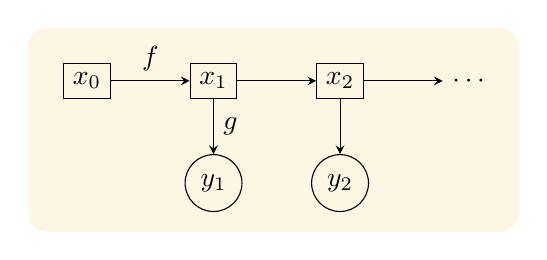
\begin{tikzpicture}[scale=1, transform shape]
    \node[draw] (x0) {$x_0$};
    \node[draw, right=of x0] (x1) {$x_1$};
    \node[draw, right=of x1] (x2) {$x_2$};
    \node[right=of x2] (x3) {$\cdots$};

    \node[draw, circle, below=2em of x1] (y1) {$y_1$};
    \node[draw, circle, below=2em of x2] (y2) {$y_2$};

    \path[-stealth]
    (x0) edge node[above] {$f$} (x1)
    (x1) edge  (x2)
    (x2) edge  (x3)
    (x1) edge node[right] {$g$} (y1)
    (x2) edge  (y2);

    \begin{pgfonlayer}{background}
        \filldraw [line width=5mm,join=round,sbase3] (x0.north west) ++ (-2mm,2mm) rectangle
        (y2.south -| x3.east);
    \end{pgfonlayer}
\end{tikzpicture}
\end{center}

        \end{column}
        \begin{column}{0.5\textwidth}
            \begin{itemize}
                
                \item Model with hidden state.

        \item Known process.

        \item Emits observables (likelihood)

        \item Combine observations and knowledge of process to find hidden state.
            \end{itemize}
        \end{column}
    \end{columns}
\end{frame}

\begin{frame}[fragile]{Probabilistic programming}
    \begin{columns}
        \begin{column}{0.5\textwidth}
 \begin{center}
 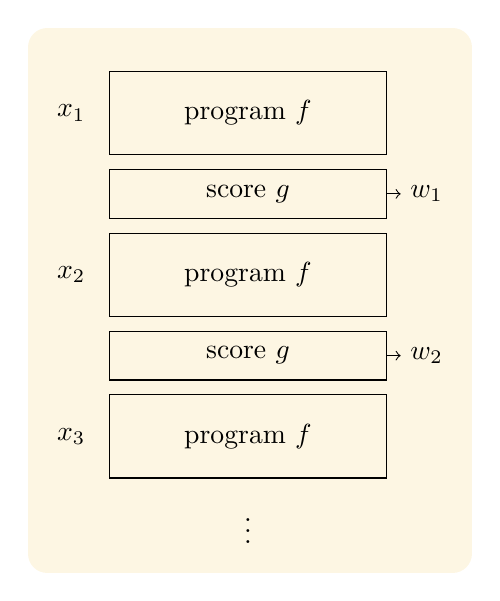
\begin{tikzpicture}[scale=1, transform shape,node distance=0.5em]
     \node[minimum width=10em,minimum height=3em,draw] (x1) {program $f$};
     \node[minimum width=10em,draw,below=of x1,inner sep=2mm] (y1) {score $g$};
     \node[minimum width=10em,minimum height=3em,draw,below=of y1] (x2) {program $f$};
     \node[minimum width=10em,draw,below=of x2,inner sep=2mm] (y2) {score $g$};
     \node[minimum width=10em,minimum height=3em,draw,below=of y2] (x3) {program $f$};
 
     \node[left=of x1] {$x_1$};
     \node[left=of x2] {$x_2$};
     \node[left=of x3] (xx3) {$x_3$};
 
     \node[right= of y1] (w1) {$w_1$};
     \node[right= of y2] (w2) {$w_2$};
 
     \node[below=of x3] (dots) {$\vdots$};
 
     \path[->]
     (y1) edge (w1)
     (y2) edge (w2);
 
     \begin{pgfonlayer}{background}
        \filldraw [line width=5mm,join=round,sbase3] (x1.north -| w1.east) ++ (0,3mm) rectangle
        (dots.south -| xx3.west);
     \end{pgfonlayer}
\end{tikzpicture}
\end{center}
        \end{column}
        \begin{column}{0.5\textwidth}
            \begin{itemize}
                \item Evolves through execution.

                \item Report likelihood for observations.
            \end{itemize}
        \end{column}
    \end{columns}
\end{frame}

\section{Monad-Bayes}
\label{sec:theory}

\begin{frame}[fragile]{Monad-Bayes implementation}
A typeclass for randomness
\begin{minted}{Haskell}
class Monad m => MonadSample m where
  random :: m Double
\end{minted}

\bigskip

A typeclass for reporting likelihood

\begin{minted}{Haskell}
class Monad m => MonadCond m where
  score :: Double -> m ()
\end{minted}

\bigskip

A typeclass for monads supporting both

\begin{minted}{Haskell}
class (MonadSample m, MonadCond m) => MonadInfer m
\end{minted}
\end{frame}

\begin{frame}[fragile]{Typeclass \texttt{MonadSample}}
A few unconditional instances:
\begin{minted}{Haskell}
newtype Enumerator a = ... -- Exhaustive enumeration
instance MonadSample Enumerator where ...
\end{minted}
\begin{minted}{Haskell}
newtype SampleIO   a = ... -- Randomness from IO
instance MonadSample SampleIO   where ...
\end{minted}

\bigskip

Allows sampling from various distributions.

Determined by how the computation is performed (\texttt{sampleIO}, \texttt{enumerate}, etc.).
\end{frame}

\begin{frame}[fragile]{Typeclass \texttt{MonadCond}}
Likelihood, the heart of Bayesian inference.

If a monad supports reporting likelihood, it \emph{cannot} be sampled from!\begin{minted}{Haskell}
result <- sampleIO model -- Error
\end{minted}
Cannot directly sample from the posterior!

Inference have to be performed!

\begin{minted}{Haskell}
-- Sample from the posterior
infer :: (MonadInfer m, MonadSample n) => m a -> n a
infer model = do ...
\end{minted}
\end{frame}

\begin{frame}[fragile]{Monad transformers}
\begin{minted}{Haskell}
-- Accumulate likelihood
newtype Weighted m a =
  Weighted (StateT (Log Double) m a)
    
-- Randomness lifted from the base monad
instance MonadSample m => MonadInfer (Weighted m)

-- Likelihoods are multiplied
instance Monad m => MonadCond (Weighted m) where
  score w = Weighted (modify (* w))
\end{minted}
\end{frame}

\begin{frame}[fragile]{Monad transformers}
\begin{minted}{Haskell}
-- Model run serveral times
newtype Population m a =
  Population (Weighted (ListT m) a)

-- Inference that may be paused
newtype Sequential m a =
  Sequential (Coroutine (Await ()) m a)
\end{minted}
\end{frame}

\section{Inference}

\begin{frame}[fragile]{SMC}
    \begin{columns}
        \begin{column}{0.5\textwidth}
    \begin{center}
        
        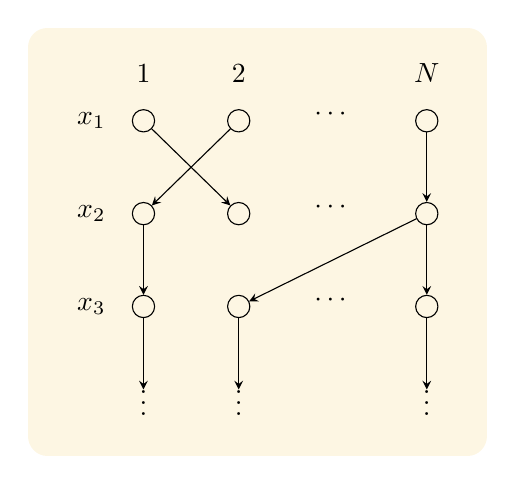
\begin{tikzpicture}[node distance=0.6em, transform shape,smcnode/.style={circle,draw,inner sep=1mm}]
    \matrix (m) [matrix of nodes,nodes in empty cells, nodes={smcnode}, row sep=1.2em, column sep=1.2em]
    {  &  & \node[draw=none] {$\cdots$};  &  \\
       &  & \node[draw=none] {$\cdots$};  &  \\
       &  & \node[draw=none] {$\cdots$};  &  \\
      \node[draw=none] {$\vdots$}; &\node [draw=none]{$\vdots$}; & \node[draw=none] {}; & \node [draw=none]{$\vdots$}; \\
      };

      \path[-stealth]
      (m-3-4) edge ++(0,-3em)
      (m-3-2) edge ++(0,-3em)
      (m-3-1) edge ++(0,-3em)
      (m-2-4) edge (m-3-4)
      (m-2-4) edge (m-3-2)
      (m-2-1) edge (m-3-1)
      (m-1-4) edge (m-2-4)
      (m-1-1) edge (m-2-2)
      (m-1-2) edge (m-2-1);

      \node[left=of m-1-1] {$x_1$};
      \node[left=of m-2-1] {$x_2$};
      \node[left=of m-3-1] {$x_3$};

      \node[above=of m-1-1] {$1$};
      \node[above=of m-1-2] {$2$};
      \node[above=of m-1-4] {$N$};

    \begin{pgfonlayer}{background}
        \filldraw [line width=5mm,join=round,sbase3] (m.north west) ++ (-2em,1em) rectangle
        (m.south east);
    \end{pgfonlayer}
\end{tikzpicture}
    \end{center}
        \end{column}
        \begin{column}{0.5\textwidth}
            Sequential Monte Carlo
            \begin{itemize}
                \item Runs the program several times.
                \item At each likelihood report: \emph{resample} trajectories.
                \item Conditional variant (CSMC) uses given extra trajectory.
            \end{itemize} 

        \end{column}
    \end{columns}

    \bigskip\centering

    SMC (exploration) $\longleftrightarrow$ CSMC (exploitation)

\end{frame}

\begin{frame}[fragile]{iPMCMC}
    \textbf{Interacting particle Markov Chain Monte Carlo}

    \bigskip

    \begin{itemize}
        
        \item MCMC-method for Bayesian inference by Rainforth et al. in their paper \emph{``Interacting Particle Markov Chain Monte Carlo''}.

\item Combination of SMC-methods.

\item Balance exploration of SMC with exploitation of CSMC.

\item Highly parallelisable.
    \end{itemize}

\end{frame}

\begin{frame}[fragile]{iPMCMC structure}
    \begin{itemize}
        
        \item \alert{$M$} SMC nodes (say 32).

\item \alert{$N$} particles par node (say 100).

\item \alert{$R$} MCMC-steps (as many as possible).

\item Half of nodes are CSMC.

\item CSMC receives trajectoy from previous step.

\item Nodes alternate.

\item Samples from CSMC nodes collected.
    \end{itemize}
    
\end{frame}

\begin{frame}[fragile]{Alternation}
    At each step, half are CSMC. Not necessarily the same half.

    Each CSMC node is resampled (with itself and SMC nodes) on marginal likelihood $\hat Z$.

    Pool of SMC includes nodes switched out earlier.
\end{frame}


\begin{frame}[fragile]{iPMCMC structure}
    \begin{center}
        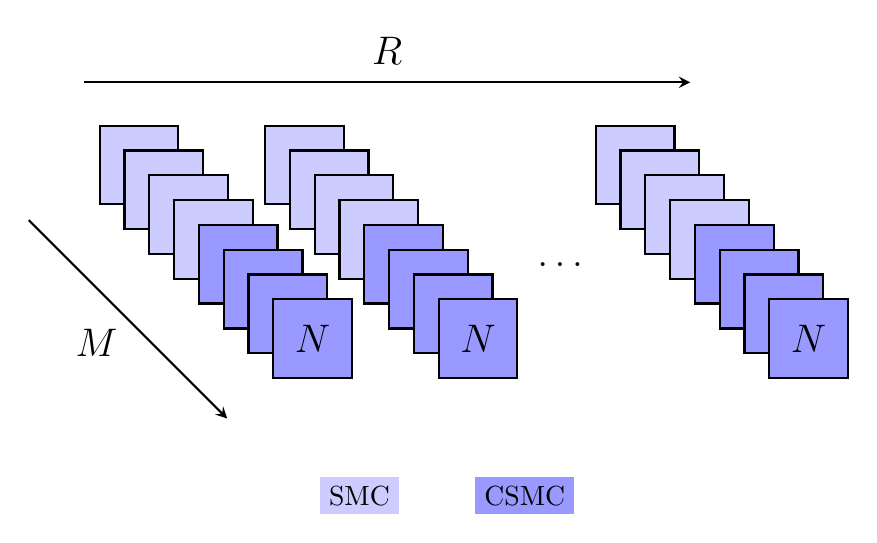
\begin{tikzpicture}[scale=0.7]
            \def\ofs{0.45}
            \foreach \x in {0,1,2,3} {
                \node[draw,thick,minimum size=1cm,fill=blue!20] at (\x*\ofs,-\x*\ofs) {};
        }
            \foreach \x in {4,5,6,7} {
                \node[draw,thick,minimum size=1cm,fill=blue!40] at (\x*\ofs,-\x*\ofs) {};
        }
        \node[] at (7*\ofs,-7*\ofs) {\Large $N$};
            \foreach \x in {0,1,2,3} {
                \node[draw,thick,minimum size=1cm,fill=blue!20] at (\x*\ofs+3,-\x*\ofs) {};
        }
            \foreach \x in {4,5,6,7} {
                \node[draw,thick,minimum size=1cm,fill=blue!40] at (\x*\ofs+3,-\x*\ofs) {};
        }
        \node[] at (7*\ofs+3,-7*\ofs) {\Large $N$};
            \foreach \x in {0,1,2,3} {
                \node[draw,thick,minimum size=1cm,fill=blue!20] at (\x*\ofs+9,-\x*\ofs) {};
        }
            \foreach \x in {4,5,6,7} {
                \node[draw,thick,minimum size=1cm,fill=blue!40] at (\x*\ofs+9,-\x*\ofs) {};
        }
        \node[] at (7*\ofs+9,-7*\ofs) {\Large $N$};

        \draw[-stealth,thick] (-1,1.5) -- node[above=0.1cm] {\Large $R$} (10,1.5);
        \draw[-stealth,thick] (-2,-1) -- node[below left] {\Large $M$} (8*\ofs-2,-8*\ofs-1);

        \node at (7.7,-1.8) {\Large\dots};

        \node[fill=blue!20] at (4,-6) {SMC};
        \node[fill=blue!40] at (7,-6) {CSMC};
        \end{tikzpicture}
    \end{center}
    
\end{frame}

\begin{frame}[fragile]{Algorithm}
    Result kept in $x'$.
    \begin{enumerate}
        \item For each MCMC iteration $1 \leq r \leq R$:
            \begin{enumerate}
                \item Run SMC nodes.
                \item Run CSMS nodes with trajectories $x'[r-1]$.
                \item For each conditional node:
                    \begin{enumerate}
                        \item Choose new conditional node.
                        \item Sample to $x'_i[r]$ from that node.
                    \end{enumerate}
            \end{enumerate}
    \end{enumerate}
\end{frame}

\section{Implementation}
\label{sec:implementation}

\begin{frame}[fragile]{SMC implementation}
    
\begin{itemize}
    \item Monad-Bayes SMC lacks functionality $\Rightarrow$ custom implementation.

    \item Custom monad with \texttt{Coroutine} and \texttt{Weighted} to collect likelihoods and suspend when reporting (for resampling).

    \item Multinomial resampling.

    \item Collect estimated marginal likelihood.

    \item CSMC only differs in resample step.

\end{itemize}
\end{frame}

\begin{frame}[fragile]{iPMCMC implementation}
    \begin{itemize}
    \item Fork \texttt{IO} to evaluate the nodes in parallel.
    \item Recurse over the results from the CSMC nodes.
    \item Resample from the current node $m$ and the rest using $\hat Z$.
    \item If necessary, update the SMC results with the switched out node.
    \item Sample trajectory $i$ on $w_{T,m}^i$.
    \item Collect samples from and conclude the MCMC step.
    \end{itemize}
\end{frame}

\section{Testing}
\label{sec:testing}

\begin{frame}[fragile]{Setup}
    Evaluate \alert{correctness} and \alert{performace} compared to other methods.

    Tested methods are:
    \begin{itemize}
        \item iPMCMC
        \item iPMCMC variants
        \item SMC
        \item Trivial parallel construct of SMC methods
    \end{itemize}
\end{frame}

\begin{frame}[fragile]{Parallelisation}
    iPMCMC with $M = 32, N = 100$ and $R = 10$.    

    Tested on 32-core AMD Opteron 6274 (\texttt{gullviva@it.uu.se}).

    Average over 10 measurements for 1--32 threads.

\end{frame}

\begin{frame}[fragile]{Amdahl's Law}
    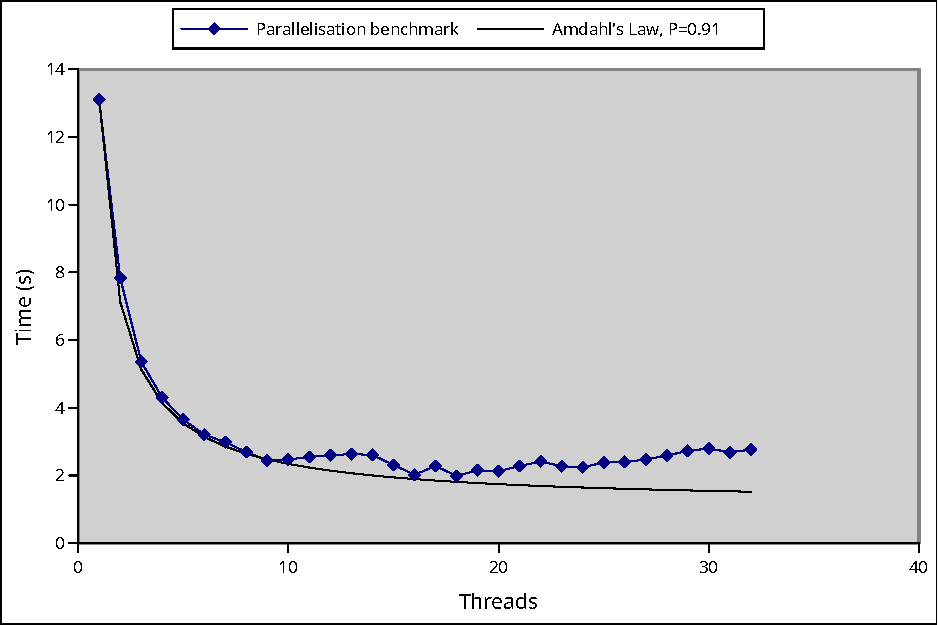
\includegraphics[width=0.45\textwidth]{parallel1.pdf}\hfill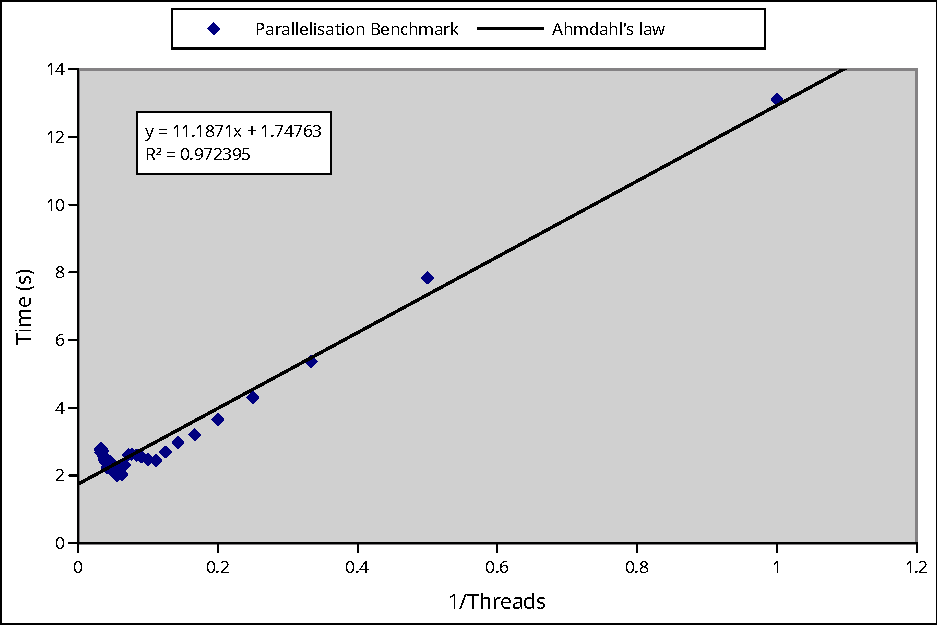
\includegraphics[width=0.45\textwidth]{parallel2.pdf}

    \[
        T(k) = T(1)\left((1-P) + \frac 1 k P\right) \Rightarrow \mathbf{ P \approx 86\%}
    \]
    
\end{frame}

\begin{frame}[fragile]{Correctness}
    iPMCMC with $M = 32, N = 100$ and $R = 1000$.    

    SMC with $N = 4096$.

    Use simple discreete model, exact posterior known.

    Compare KL-divergence between the exact and calculated posterior.

    It should be a straight line on a log-log plot.
\end{frame}

\begin{frame}[fragile]{Correctness}
    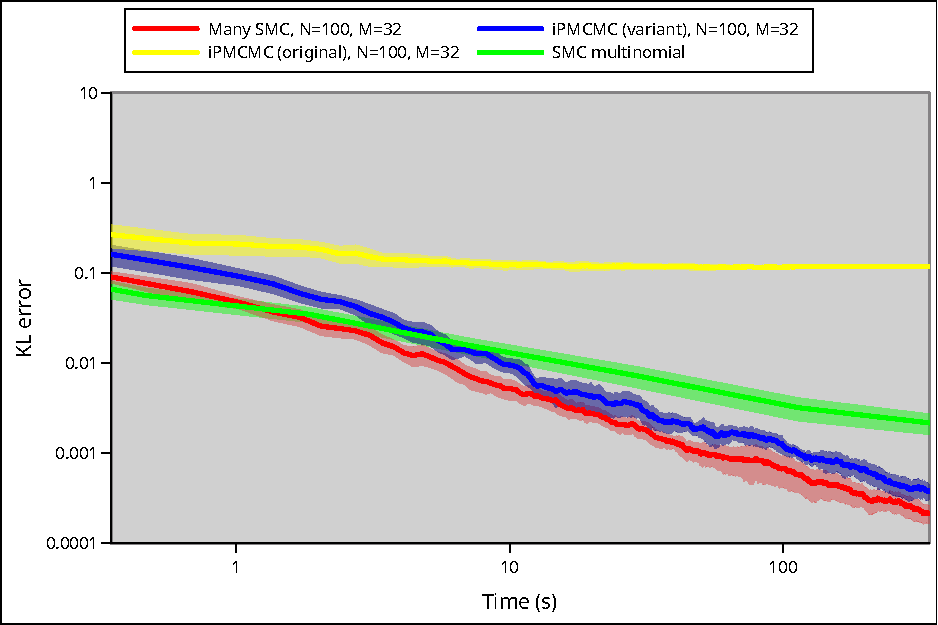
\includegraphics[width=\textwidth]{correctness.pdf}
\end{frame}

\begin{frame}[fragile]{Correctness}
    \begin{columns}
        \begin{column}{0.5\textwidth}
    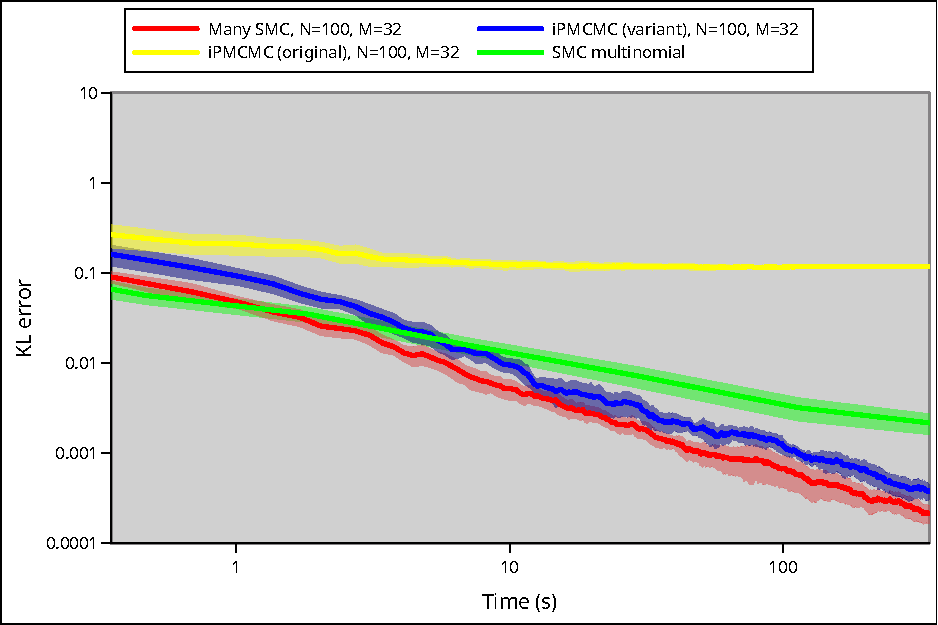
\includegraphics[width=\textwidth]{correctness.pdf}
        \end{column}
        \begin{column}{0.5\textwidth}
            \begin{itemize}
                \item My iPMCMC not correct (33 MB).
                \item Variant iPMCMC correct (659 MB).
                \item Monad-Bayes SMC (12 MB).
                \item Many SMC (3121 MB).
            \end{itemize} 
        \end{column}
    \end{columns}
\end{frame}

\section{Results}
\label{sec:results}



\begin{frame}[fragile]{Evaluation}
    \begin{itemize}
        \item Parallelisation good! Over 80\%.
        \item Implementation not correct\dots
        \item Variant is! Points to bug location.
        \item Many SMC better $\Rightarrow$ not true potential.
        \item SMC outperformed after a few seconds.
    \end{itemize}
\end{frame}

\begin{frame}[fragile]{Limitations \& Future}
    \begin{itemize}
        \item Does not support all models.
        \item Does not use Rao-Blackwellisation to improve quality.
        \item Most certainly room for Haskell-side optimisations.
    \end{itemize}
    \begin{itemize}
        \item Few models tested.
        \item Does not test against iPMCMC implementation in Anglican.
        \item Simple model tested.
    \end{itemize}
\end{frame}

\begin{frame}{The End}
    \centering
    \Huge Questions?
\end{frame}

\end{document}
